\documentclass[12pt,a4paper]{article}
\pdfminorversion=7

\usepackage[british]{babel}
\usepackage[a4paper,top=2cm,bottom=2cm,left=2.5cm,right=2.5cm,marginparwidth=1.75cm]{geometry}
\usepackage[style=apa, backend=biber]{biblatex}
\addbibresource{references.bib}
\DeclareLanguageMapping{british}{british-apa}
\DeclareFieldFormat[article]{volume}{\apanum{#1}}
\renewcommand*{\finalnamedelim}{%
  \ifnumgreater{\value{liststop}}{2}{\finalandcomma}{}%
  \addspace\&\space}

\usepackage{amsmath}
\usepackage{graphicx}
\usepackage[colorlinks=true, allcolors=blue]{hyperref}
\usepackage{booktabs}
\usepackage{threeparttable}
\usepackage{subcaption}
\usepackage{authblk}
\usepackage[T1]{fontenc}
\usepackage{csquotes}
\usepackage{url}
\usepackage{helvet}
\usepackage{lmodern}
\usepackage{setspace}
\usepackage{titlesec}
\usepackage{caption}
\usepackage{float}
\onehalfspacing
\setlength{\emergencystretch}{3em}

\titleformat{\section}{\normalfont\Large\bfseries}{\thesection.}{1em}{}
\captionsetup[table]{position=top,labelfont=bf}
\captionsetup[figure]{labelfont=bf}
\date{}

\begin{document}

\begin{center}
{\Huge Style-induced volumetric contraction in TripoSR:}
\\[1.5ex]
{\Large A controlled benchmark of stylised input transformations}
\\[5ex]

{\large Wei Xiong$^{1}$, Wei Meng$^{2}$, Chu Qiu$^{3,*}$, and ShuWen Li$^{1}$}
\\[1.5ex]
{\small
$^{1}$Guilin Institute of Information Technology, Guilin, Guangxi, China \\
$^{2}$Guilin Normal College, Guilin, Guangxi, China \\
$^{3}$Guilin Life and Health Career Technical College, Guilin, Guangxi, China \\
$^{*}$Corresponding author: Chu Qiu, \href{mailto:appamm94@gmail.com}{appamm94@gmail.com} \\
E-mail addresses: Wei Xiong, \href{mailto:xiongwei@guit.edu.cn}{xiongwei@guit.edu.cn};
Wei Meng, \href{mailto:mengwei@mail.glnc.edu.cn}{mengwei@mail.glnc.edu.cn};
ShuWen Li, \href{mailto:lishuwen@guit.edu.cn}{lishuwen@guit.edu.cn}.
}
\end{center}

\begin{abstract}
Single-image 3D reconstruction is increasingly used to turn visual concepts into editable assets, but evaluation still relies heavily on surface-distance metrics. We study what changes when TripoSR reconstructs the same object from matched photographic and stylised renderings. The benchmark contains 100 curated Objaverse objects, each rendered as one photo input and five controlled artistic-style proxies, giving 600 reconstructions under an identical pipeline. Every stylised condition reduces predicted mesh volume relative to its paired photo output: mean volume ratios range from 0.257 for sketch to 0.500 for flat colour, with paired Wilcoxon tests below $10^{-16}$. Aggregate Chamfer and F-score values improve for several styles, creating an apparent disagreement between surface proximity and volumetric preservation. A post hoc sensitivity analysis shows that these F-score gains are concentrated among objects with weak photo reconstructions. In the top quartile of photo-baseline F-score, the mean F-score change is negative for every style, whereas volumetric contraction remains. A 30-object rerun at marching-cubes resolution 128 preserves the contraction pattern. The evidence therefore supports two distinct conclusions: stylisation systematically changes the volume of TripoSR outputs in this benchmark, while apparent surface-metric gains depend on baseline quality. Image-to-3D evaluation for design workflows should report paired volume and depth diagnostics alongside Chamfer and F-score.
\end{abstract}

\textbf{Keywords}: image-to-3D, TripoSR, stylised inputs, geometry evaluation, volumetric contraction, benchmark.

\section{Introduction}

Single-image 3D reconstruction has moved from a specialised vision problem into a practical tool for design, game production, digital heritage, and AI-assisted asset generation. Recent systems can produce a mesh from one image in seconds or minutes, and large reconstruction models have made this workflow much easier to deploy \parencite{hong2023lrm,tochilkin2024triposr,xu2024instantmesh}. The same shift is now visible in adjacent design tasks, including AI-assisted CAD generation and single-image reconstruction for cultural heritage \parencite{doris2026cadbench,wu2026culturalrelics}. In these settings, the input image is not always a clean photograph. Artists and designers often begin with sketches, flat illustrations, low-detail thumbnails, stylised concept art, or watercolour-like references. A 3D generator that appears robust on natural images may therefore behave differently when the visual evidence is intentionally abstract.

The usual evaluation protocol does not fully expose this problem. A reconstructed mesh can score well under Chamfer distance or F-score because its visible surface lies close to the sampled ground-truth surface, even when the object has lost volume, thickness, or usable back-side structure. For engineering and design use, these failures matter. A thin shell, flattened body, or collapsed depth profile may be a poor 3D asset even if a point-cloud metric improves. The issue is sharper for artistic inputs because style transformations often remove texture, compress shading, simplify boundaries, or emphasise contours. These changes can make the input easier for a metric that favours visible outline alignment while making the recovered object less useful as geometry.

This mismatch is not merely a visual-quality concern. Many image-to-3D systems are now presented as asset-generation tools rather than as point-cloud predictors. The output may be remeshed, sculpted, textured, animated, inserted into a game engine, used as a design reference, or passed to a fabrication-oriented workflow. In such cases, a mesh that is topologically simple but volumetrically collapsed can be more damaging than a mesh with modest surface noise. It may look acceptable from the source view but fail when rotated, edited, or interpreted as a solid object. This is why an evaluation protocol that reports only surface proximity can be misleading for computational design.

Artistic inputs make the problem unusually testable. A sketch, flat-colour rendering, or watercolour image removes some visual cues while preserving others. Contours may remain sharp even when shading and texture are gone; a flat illustration may retain semantic identity while suppressing depth evidence; a low-detail image may preserve global silhouette while erasing local geometry. If the same underlying object is reconstructed from both a photographic rendering and a stylised rendering, the paired difference can reveal which part of the reconstruction is robust to abstraction and which part depends on photographic cues. This paired design is stronger than comparing unrelated photographs and artworks because it fixes object identity, pose, camera view, and ground-truth geometry.

This paper studies that mismatch through a controlled benchmark. Instead of collecting unrelated photographs and artworks, we start from known 3D objects. Each object is rendered into a photographic reference and five matched artistic variants: edge, flat colour, low-detail, sketch, and watercolour. This paired design keeps the underlying object fixed, keeps the 3D ground truth available, and isolates the effect of input style. We then run the same image-to-3D model, TripoSR \parencite{tochilkin2024triposr}, on every input and compare each stylised reconstruction with the corresponding photo reconstruction.

The main finding has two parts. On 100 Objaverse objects \parencite{deitke2022objaverse}, every stylised condition reduces predicted mesh volume relative to the photo input. The mean volume ratios are 0.332 for edge, 0.500 for flat colour, 0.305 for low-detail, 0.257 for sketch, and 0.343 for watercolour. Aggregate surface metrics can nevertheless improve: sketch, for example, increases mean F-score@0.05 by 0.093 and reduces Chamfer distance by 0.010. However, a baseline-quality sensitivity analysis shows that these gains are concentrated among objects for which the photo reconstruction is already weak. Volumetric contraction persists when the analysis is restricted to the stronger half of photo baselines.

Our contribution is not a new image-to-3D generator. It is an evaluation and diagnostic study of one open, widely used baseline under controlled input shifts. We make three contributions. First, we define a paired cross-style benchmark in which photographic and stylised inputs share the same object, camera view, and known 3D ground truth. Second, we show a consistent volumetric contraction in TripoSR outputs, including strong reductions in volume and z-extent. Third, we separate the robust volumetric result from a conditional metric paradox: aggregate Chamfer and F-score gains are moderated by photo-baseline quality. The result suggests that evaluation for computational design and 3D asset generation should treat volumetric diagnostics as first-class evidence rather than optional visual checks.

The paper is organised as follows. Section~2 reviews single-image 3D reconstruction, artistic or sketch-based 3D generation, and recent evaluation work. Section~3 describes the paired benchmark, the reconstruction protocol, and the metric design. Section~4 reports the main 100-object experiment and the higher-resolution robustness rerun. Section~5 discusses the implications for benchmarking and design workflows, and Section~6 summarises the main limitations.

\section{Related work}

\subsection{Datasets and generative priors for 3D reconstruction}

The recent acceleration of image-to-3D research depends on two ingredients: large 3D object corpora and generative priors learned from 2D or multi-view data. Objaverse made a large collection of annotated 3D objects available for training and evaluation \parencite{deitke2022objaverse}, and Objaverse-XL expanded the scale by more than an order of magnitude \parencite{deitke2023objaversexl}. More recent curation work adds quality annotations and filtering signals for object-level datasets \parencite{lin2025objaversepp}. These resources make it possible to build controlled benchmarks in which the image input is generated from known 3D geometry rather than collected from unrelated web images.

This distinction matters for evaluation. Web images and artworks often differ in object category, viewpoint, scene context, lighting, and level of abstraction. A comparison across such images can easily confound model sensitivity to style with ordinary differences in content. Large object corpora make a cleaner design possible: one can render the same mesh under different visual conditions and then measure all reconstructions against the same ground truth. The present benchmark follows this controlled-evaluation logic. It uses Objaverse as a source of object geometry, but it does not treat the dataset itself as the contribution. The contribution is the paired style manipulation and the metric analysis that becomes possible once the object is fixed.

Large 3D corpora also shape the models being evaluated. Several recent reconstruction models are trained on synthetic or rendered views of large object collections, so their behaviour depends on what kinds of cues are common in those training views. If a model has mainly learned from naturalistic renderings, it may infer depth from shading, texture gradients, and photographic appearance. A stylised image can remove precisely those cues. The benchmark therefore probes a realistic distribution shift: the object remains familiar, but the evidence available to the reconstruction model changes.

\subsection{Single-image 3D generation and large reconstruction models}

Single-image 3D generation has moved from optimisation-heavy pipelines toward feed-forward reconstruction. Zero-1-to-3 learns view-conditioned generation from one image \parencite{liu2023zero123}; One-2-3-45 and One-2-3-45++ combine view generation and reconstruction to produce meshes quickly \parencite{liu2023one2345,liu2023one2345pp}. Wonder3D introduced cross-domain diffusion for single-image 3D generation, and Wonder3D++ extends the same line toward higher-fidelity results \parencite{long2023wonder3d,long2025wonder3dpp}. Large reconstruction models such as LRM, TripoSR, InstantMesh, and CRM further reduce inference time or improve sparse-view reconstruction quality \parencite{hong2023lrm,tochilkin2024triposr,xu2024instantmesh,wang2024crm}.

The field has continued to move quickly after these early large reconstruction models. MeshLRM, Unique3D, MeshFormer, GS-LRM, LRM-Zero, GeoLRM, and multi-view LRM variants explore higher-quality mesh generation, Gaussian reconstruction, synthetic-data training, and geometry-aware positional encoding \parencite{wei2024meshlrm,wu2024unique3d,liu2024meshformer,zhang2024gslrm,xie2024lrmzero,zhang2024geolrm,li2024mvlrm}. More recent work, including NOVA3D, Cue3D, MAGE, and UniMesh, shifts attention toward normal-aligned video diffusion, image-cue attribution, material-aware 3D generation, and joint mesh understanding/generation \parencite{yang2025nova3d,li2025cue3d,wang2025mage,huang2026unimesh}. This rapid progress makes evaluation more important, not less: a model can be fast and visually plausible while still failing under input conditions that are common in design practice.

Most of these systems are evaluated on natural images, synthetic multi-view renderings, or standard object benchmarks. That evaluation is necessary, but it does not answer whether a system is reliable for design sketches or illustrative concept images. TripoSR is a useful case study for this question because it is fast, open, and representative of feed-forward image-to-3D reconstruction. We use it as a diagnostic baseline rather than as the object of a model-ranking study. The results should therefore be read as evidence that the evaluation problem exists, not as a final statement about every current image-to-3D model.

\subsection{Artistic, illustrated, and sketch-based 3D inputs}

Non-photographic image-to-3D input now has its own line of work. Sketch-A-Shape studies zero-shot sketch-to-3D generation \parencite{sanghi2023sketchashape}, Sketch3D adds style-consistent guidance for sketch-driven generation \parencite{zheng2024sketch3d}, and PASTA uses part-aware priors for sketch-to-3D shape generation \parencite{lee2025pasta}. A 2026 survey on deep sketch-based 3D modelling shows that sketch-driven 3D creation has become a broad research area rather than a single-task variant \parencite{tono2026sketchsurvey}.

Other work studies more specialised stylised domains. PAniC-3D reconstructs stylised anime portraits \parencite{chen2023panic3d}; DrawingSpinUp animates single character drawings \parencite{zhou2024drawingspinup}; Art3D targets flat-coloured illustration with a training-free correction pipeline \parencite{cong2025art3d}; and a semi-automated framework for medieval manuscript miniatures evaluates several image-to-3D systems on historical illustrated inputs \parencite{pallotto2026miniatures}. Recent work also extends stylisation to reconstructed 3D assets and scenes, including 3D stylisation through large reconstruction models and language-driven artistic scene generation \parencite{oztas2025stylizationlrm,li2025artiscene}.

Our study is positioned differently from these domain-specific systems. We do not introduce a new stylised reconstruction model, nor do we claim that artistic 3D generation is unexplored. Instead, we use matched styles of the same ground-truth objects to test how input abstraction changes the measured geometry. The paired construction lets us observe metric disagreement without confounding style with object category, pose, or dataset source.

This positioning is important because specialised stylised models and general-purpose reconstruction models answer different questions. A specialised method may be designed to handle a particular artistic domain, such as anime portraits or flat-coloured illustrations. A general-purpose model may be used by practitioners because it is available, fast, and easy to run. Our benchmark asks what happens in the latter case: if a user gives a general reconstruction model a design-like input, do the standard metrics reveal the loss of usable 3D structure? The answer in our experiment is no, or at least not reliably.

\subsection{Evaluation benchmarks and the metric gap}

Evaluation for generative 3D models is beginning to receive more direct attention. 3DGen-Bench proposes a broad benchmark suite for 3D generative models \parencite{jiang2025threedgenbench}, 3D Arena provides an open platform for generative 3D evaluation \parencite{ebert2025threedarena}, and SI23DCQA studies perceptual quality assessment for single-image-to-3D content \parencite{fu2025si23dcqa}. In computational design, CADBench similarly treats generation quality as a benchmark problem rather than a single example-by-example judgement \parencite{doris2026cadbench}. These efforts reflect a wider concern: as 3D generation becomes easier to run, visual plausibility alone is not enough to certify geometric usefulness.

Chamfer distance and F-score remain useful because they are reproducible and compatible with sampled point clouds. Yet they measure surface proximity more directly than asset usability. A reconstruction can place many sampled points close to a ground-truth surface while losing volume, thickness, back-side plausibility, or connected structure. For computational design and engineering workflows, the mesh is not only an image surrogate. It may be edited, remeshed, textured, animated, fabricated, or used as a proxy for downstream analysis. A flattened mesh is therefore a different failure from a small surface offset. The present benchmark treats volume, z-extent, and mesh-complexity ratios as diagnostic signals that complement point-distance metrics.

Recent benchmark work points in the same direction. 3DGen-Bench and 3D Arena broaden evaluation beyond isolated visual examples, while SI23DCQA studies perceptual quality for single-image-to-3D outputs \parencite{jiang2025threedgenbench,ebert2025threedarena,fu2025si23dcqa}. CADBench brings a similar benchmark mentality to AI-assisted design, where executability and compactness matter in addition to geometric fidelity \parencite{doris2026cadbench}. Our work adds a narrower but practical test: when the image style changes while the object stays fixed, conventional point metrics can disagree with volume-sensitive diagnostics. That disagreement is precisely the kind of failure a design-oriented benchmark should expose.

\section{Material and methods}

\begin{figure}[!ht]
\centering
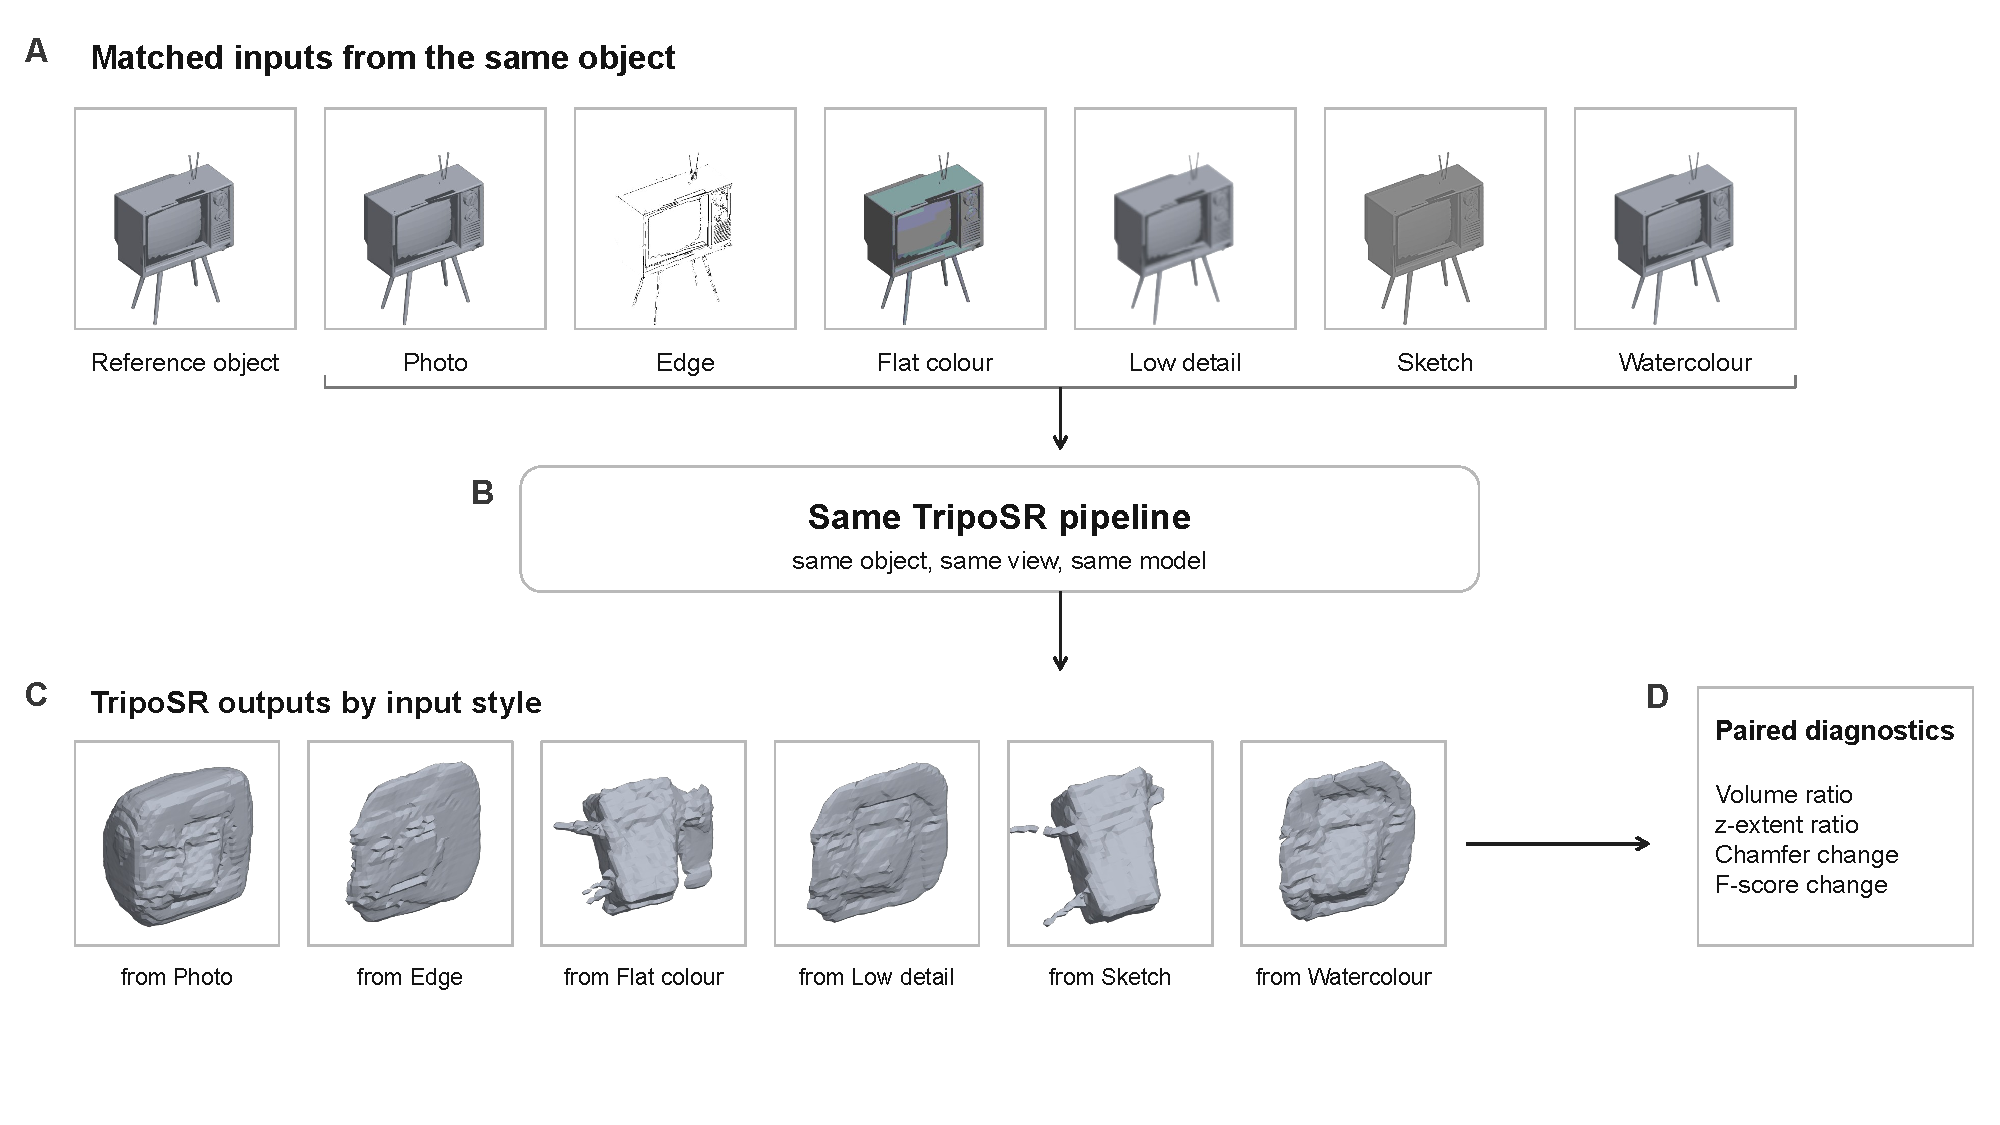
\includegraphics[width=\linewidth]{figures/fig1_framework_baseline_audited.pdf}
\caption{\label{fig:framework}Paired benchmark construction, illustrated with one preserved television sample from the experiment. (A) The reference object is rendered as a photo input and five matched controlled style variants under the same view. (B) Every input is processed by the same TripoSR pipeline without style-specific tuning. (C) The resulting meshes are rendered under a common evaluation view. (D) Each stylised reconstruction is compared with the photo reconstruction of the same object using paired surface and volumetric diagnostics.}
\end{figure}

\subsection{Object selection}

We use Objaverse as the source of ground-truth 3D objects \parencite{deitke2022objaverse}. From the available objects, we curate a 100-object subset for the main experiment. The curation removes very large meshes, extremely low-complexity meshes, obvious intellectual-property or trademarked objects, human figures, full scenes, and collection-like samples. We also retain only permissively licensed objects marked as BY or BY-SA in the run manifest. This keeps the benchmark small enough to reproduce while avoiding many cases where reconstruction failure would be caused by object ambiguity rather than style.

The subset is deliberately modest. The aim is not to approximate the full diversity of Objaverse, but to create a controlled diagnostic benchmark that can be rerun on affordable hardware. Each selected object is treated as a unit of paired comparison. The same object contributes one photo reconstruction and five stylised reconstructions, so the statistical test is based on within-object changes rather than on differences between object categories. This design reduces variance from mesh complexity, object identity, and pose. It also makes the results easier to interpret: a volume ratio below one means that the stylised input produced a smaller mesh than the photo input for the same object.

During curation we prioritised objects that could be rendered as recognisable single-object inputs. Full scenes, assemblies with many disconnected parts, and objects whose identity depended on fine text or brand marks were removed. These cases are important in practice, but they introduce additional failure modes that are not the focus of this paper. The benchmark instead asks a narrower question: even for relatively clean object-level inputs, does artistic abstraction change the geometry recovered by an image-to-3D model?

\subsection{Matched input styles}

For each object, we render a photographic input and five stylised variants. These variants are controlled artistic-style proxies rather than samples of unconstrained human artwork. The style set covers several common forms of visual abstraction while keeping object identity and viewpoint fixed:
\begin{itemize}
    \item \textbf{photo}: the reference input used as the paired baseline;
    \item \textbf{edge}: a contour-dominant rendering with reduced interior evidence;
    \item \textbf{flat}: a flat-colour version with simplified shading;
    \item \textbf{low-detail}: a simplified rendering with reduced visual detail;
    \item \textbf{sketch}: a hand-drawing-like abstraction;
    \item \textbf{watercolour}: a soft stylised rendering with diffuse boundaries and colour variation.
\end{itemize}
The important property is pairing. Each stylised input corresponds to the same underlying mesh and view as its photo counterpart. This lets us report relative changes style by style instead of comparing unrelated images.

The five stylised variants were chosen to cover different forms of abstraction rather than to reproduce one named artistic school. Edge inputs preserve outline information while discarding much of the interior appearance. Flat-colour inputs preserve object regions but reduce shading gradients. Low-detail inputs suppress local texture and small-scale visual evidence. Sketch inputs emphasise drawn contours and sparse strokes. Watercolour inputs retain colour variation but soften boundaries and local contrast. These transformations are not intended to exhaust the space of artistic images. They provide a compact set of controlled perturbations that resemble common inputs in early-stage design and illustration workflows.

All styles are derived from the same source-object rendering and share the same view as the photo input. This is essential because a different view would change the amount of visible geometry and make the paired comparison ambiguous. The photo input is used as the baseline because it represents the input type for which many image-to-3D systems are most commonly demonstrated. We do not treat the photo reconstruction as ground truth. Ground truth remains the original 3D object. The photo reconstruction is used only as a within-model reference for asking how much a style transformation changes the model output.

\subsection{Reconstruction protocol}

All 600 inputs are reconstructed with TripoSR \parencite{tochilkin2024triposr}. We use TripoSR because it is a fast, open image-to-3D baseline and can process the full benchmark at modest cost. The goal is not to rank models; it is to test whether a widely used reconstruction pipeline exhibits style-induced metric disagreement under controlled inputs. The main run reconstructs 100 objects across six styles with marching-cubes resolution 64. All 600 reconstructions succeed and produce watertight output meshes.

To check whether the observed volume reduction is merely caused by the mesh-extraction resolution, we run a separate 30-object robustness experiment with marching-cubes resolution increased to 128. This rerun covers the same six styles and produces 180 successful reconstructions.

The reconstruction protocol is intentionally held constant across styles. We do not tune model parameters separately for sketch, flat, watercolour, or photo inputs. Style-specific tuning would make it difficult to determine whether the measured differences come from the input or from the intervention. The same pipeline therefore receives each rendered image, produces a mesh, and passes the mesh to the same evaluation scripts. This fixed-pipeline design mirrors a common user workflow: a practitioner selects a general image-to-3D model and applies it to whatever reference image is available.

The robustness rerun addresses a simple concern. If the main experiment used a low mesh-extraction resolution, then a smaller or thinner mesh might be an artefact of the extraction grid rather than of the reconstruction itself. Increasing the marching-cubes resolution cannot prove that no extraction artefact remains, but it can test whether the qualitative pattern disappears under a denser extraction. In our rerun it does not disappear. We therefore interpret the higher-resolution run as evidence that the observed shrinkage is not only a low-resolution extraction effect.

\subsection{Metrics}

We compute conventional point metrics against the ground-truth object, including Chamfer L2 and F-score at 0.05 and 0.1 thresholds. The evaluation samples 50,000 surface points from each ground-truth object and 30,000 points from each predicted mesh, followed by the same bounding-box normalisation and alignment procedure for every style. Chamfer distance measures average point proximity; F-score measures how many sampled points fall within a chosen tolerance. Both are useful, but both are most directly about surface proximity.

We also compute diagnostics aimed at asset usability: predicted mesh volume, z-extent, vertex count, and face count. Volume captures whether the reconstruction remains a three-dimensional body rather than a thin surface. Z-extent captures loss of depth along the view-related axis. Vertex and face counts provide a coarse check on mesh complexity, although they should not be interpreted as quality measures by themselves. Most source Objaverse meshes in the curated set are not watertight, so their absolute enclosed volumes are not used as ground truth. Instead, volume is compared only between the watertight TripoSR outputs for matched photo and stylised inputs. One low-detail output has a non-finite recorded volume and is excluded from analyses involving that ratio; all other style--object pairs are retained.

For each stylised input, we report the paired change relative to the photo reconstruction of the same object. Chamfer and F-score are reported as differences, while volume and z-extent are reported as ratios. A volume ratio below 1 indicates that the stylised reconstruction has less predicted volume than the paired photo reconstruction. A z-extent ratio below 1 indicates a shallower reconstruction. We use paired Wilcoxon signed-rank tests because the comparisons are within object and the distributions need not be Gaussian. We accompany the tests with rank-biserial effect sizes, medians, proportions below a 0.5 volume ratio, and percentile-bootstrap 95\% confidence intervals for the mean (10,000 resamples; fixed seed 20260713).

Formally, let $G_i$ denote the ground-truth object for object $i$, $x_{i,p}$ the photo input, and $x_{i,s}$ the stylised input under style $s$. The fixed reconstruction model $f$ produces meshes $M_{i,p}=f(x_{i,p})$ and $M_{i,s}=f(x_{i,s})$. We define the paired diagnostic ratios and metric changes as
\begin{align}
r^{V}_{i,s} &= \frac{V(M_{i,s})+\epsilon}{V(M_{i,p})+\epsilon}, &
r^{Z}_{i,s} &= \frac{Z(M_{i,s})+\epsilon}{Z(M_{i,p})+\epsilon}, \\
\Delta F_{i,s} &= F(M_{i,s},G_i)-F(M_{i,p},G_i), &
\Delta CD_{i,s} &= CD(M_{i,s},G_i)-CD(M_{i,p},G_i),
\end{align}
where $V(\cdot)$ is mesh volume, $Z(\cdot)$ is z-extent, $F(\cdot,\cdot)$ is F-score at the specified threshold, $CD(\cdot,\cdot)$ is Chamfer L2 distance, and $\epsilon$ is a small stabilising constant. We use the phrase metric paradox for cases where $\Delta F_{i,s}>0$ or $\Delta CD_{i,s}<0$ while $r^{V}_{i,s}$ remains far below 1.

The main analysis is therefore organised around three questions. First, do stylised inputs change conventional point metrics relative to photo inputs? Second, do the same inputs change volumetric and depth-sensitive diagnostics? Third, can these two answers disagree? The third question is the most important for this paper because it tests whether a benchmark based only on point metrics would lead to a different conclusion from a benchmark that also tracks asset-oriented geometry.

We do not normalise away the paired photo reconstruction when reporting the main diagnostic ratios, because the photo output represents the model's own baseline under the same object and camera. If a model already reconstructs an object imperfectly from the photo input, the style ratio measures the additional change caused by stylisation rather than the absolute error of the model. Absolute metrics against the ground-truth object remain part of the analysis through Chamfer and F-score, but the paired ratios are more direct for identifying style-induced contraction.

\subsection{Photo-baseline sensitivity analysis}

Aggregate differences relative to photo can be affected by the quality of the photo reconstruction itself. We therefore conduct a post hoc sensitivity analysis using the absolute F-score@0.05 of each photo reconstruction. Objects are split at the median photo F-score (0.2368) into equal lower- and higher-quality halves, and the upper quartile is examined separately. Within each stratum, we recompute the mean paired F-score change and volume ratio for every style. This analysis was not part of the original confirmatory design; it is used to determine whether the apparent surface-metric gains and the volumetric contraction have the same dependence on baseline quality.

\section{Results}

\begin{figure}[!ht]
\centering
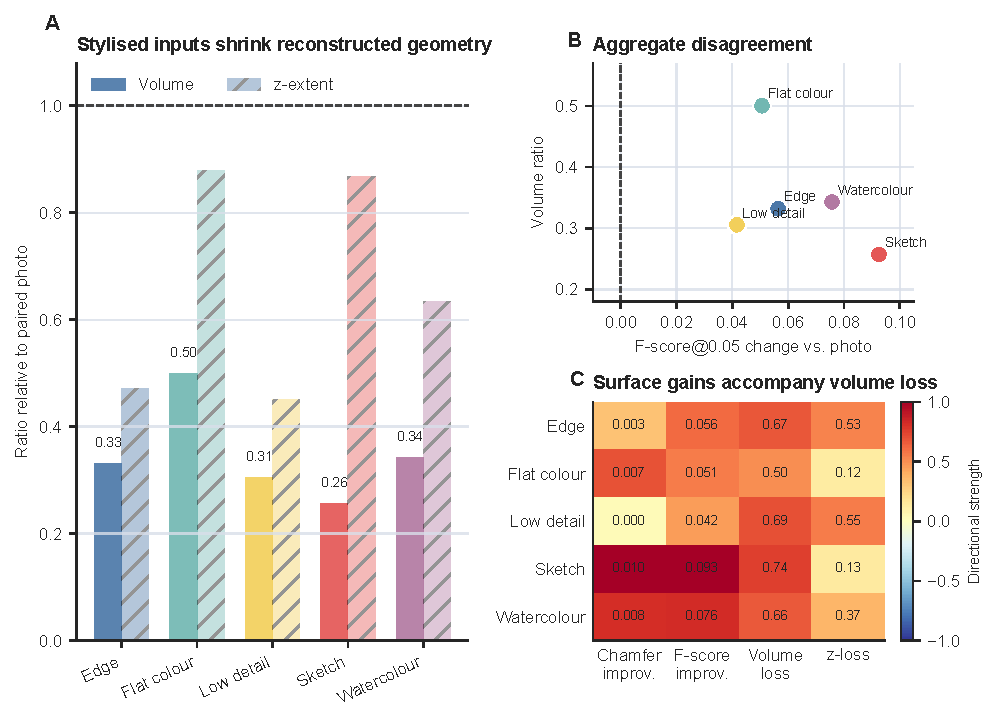
\includegraphics[width=\linewidth]{figures/fig2_main100_results.pdf}
\caption{\label{fig:main100}Main 100-object aggregate results. (A) All stylised inputs reduce predicted mesh volume relative to the paired photo reconstruction, and several also reduce z-extent. (B) Mean F-score@0.05 increases for all five styles in the unstratified analysis, although the corresponding volume ratios remain below one. (C) Reading surface and volumetric diagnostics together reveals a disagreement that is hidden by either metric family alone.}
\end{figure}

\subsection{Stylised inputs consistently reduce reconstructed volume}

Table~\ref{tab:main100} summarises the 100-object main experiment. Every stylised input reduces predicted mesh volume relative to the photo input. The largest reduction appears for sketch, with a mean volume ratio of 0.257. Low-detail and edge inputs are similarly severe, with ratios of 0.305 and 0.332. Watercolour gives a ratio of 0.343, and flat colour is less severe but still halves the predicted volume on average. The paired Wilcoxon p-values for volume are all below $10^{-16}$, and rank-biserial effect sizes range from $-0.970$ to $-1.000$.

The effect is also robust to summary choice. Median volume ratios are 0.318 for edge, 0.471 for flat colour, 0.272 for low-detail, 0.186 for sketch, and 0.304 for watercolour. The bootstrap 95\% confidence intervals for the mean are [0.305, 0.359], [0.439, 0.562], [0.276, 0.338], [0.214, 0.304], and [0.313, 0.375], respectively. The proportion of outputs below half the paired photo volume ranges from 53\% for flat colour to 94\% for low-detail. These are relative changes between model outputs, not absolute volume errors against the mostly non-watertight source meshes.

\begin{table}[!ht]
\caption{Main 100-object results relative to photo input. Negative Chamfer means lower Chamfer than photo; positive F-score means higher F-score than photo. Volume and z-extent are ratios relative to the paired photo reconstruction.}
\label{tab:main100}
\centering
\begin{tabular}{lrrrrr}
\toprule
Style & $\Delta$ Chamfer & $\Delta$ F@0.05 & Volume ratio & z-extent ratio & Volume $p$ \\
\midrule
edge & -0.0032 & 0.0564 & 0.332 & 0.471 & $3.90\times10^{-18}$ \\
flat & -0.0069 & 0.0506 & 0.500 & 0.879 & $3.75\times10^{-17}$ \\
low-detail & -0.0003 & 0.0416 & 0.305 & 0.451 & $6.44\times10^{-18}$ \\
sketch & -0.0100 & 0.0925 & 0.257 & 0.868 & $4.14\times10^{-18}$ \\
watercolour & -0.0081 & 0.0757 & 0.343 & 0.635 & $3.90\times10^{-18}$ \\
\bottomrule
\end{tabular}
\end{table}

The z-extent results show that this is not only a scale effect. Edge and low-detail inputs reduce z-extent to roughly 47\% and 45\% of the photo reconstruction, respectively. Watercolour reduces z-extent to 63\%. Flat colour and sketch preserve more z-extent on average, but they still lose substantial volume. This pattern suggests several types of collapse: some styles make the object thinner along depth, while others preserve a bounding depth but lose bulk or connected volume.

The difference between volume and z-extent is informative. Edge and low-detail inputs reduce both volume and z-extent, suggesting a depth-compression failure. Sketch inputs, by contrast, preserve more z-extent on average while producing the lowest volume ratio. This points to a different failure mode: the reconstruction may maintain a broad depth range but lose bulk within that range. Flat colour is again distinct. It produces the mildest z-extent change and the mildest volume reduction, which is consistent with the idea that flat regions preserve more object-level area information than edge-only or low-detail inputs. These distinctions would be lost if the analysis reported only a single aggregate score.

\subsection{Point metrics can improve while volumetric usability degrades}

At the aggregate level, point metrics and volumetric diagnostics disagree. Sketch reduces Chamfer by 0.0100 and increases F-score@0.05 by 0.0925 relative to the photo input, yet its mean volume ratio is only 0.257. Watercolour and flat inputs show the same aggregate direction: better Chamfer and F-score, lower volume. Edge increases mean F-score@0.05 by 0.0564 while reducing volume to one third of the paired photo reconstruction. Figure~\ref{fig:metricparadox} shows the per-object distribution and two representative sketch cases; it should be read as evidence of frequent, not universal, disagreement.

This does not mean Chamfer and F-score are wrong. It means they answer a narrower question. They can reward a reconstruction that places sampled points near the ground-truth visible surface, while missing whether the mesh remains a usable three-dimensional body. In artistic inputs, simplified contours and reduced texture may make surface alignment easier for some objects, but the model can still infer a thinner or more collapsed shape.

\begin{figure}[H]
\centering
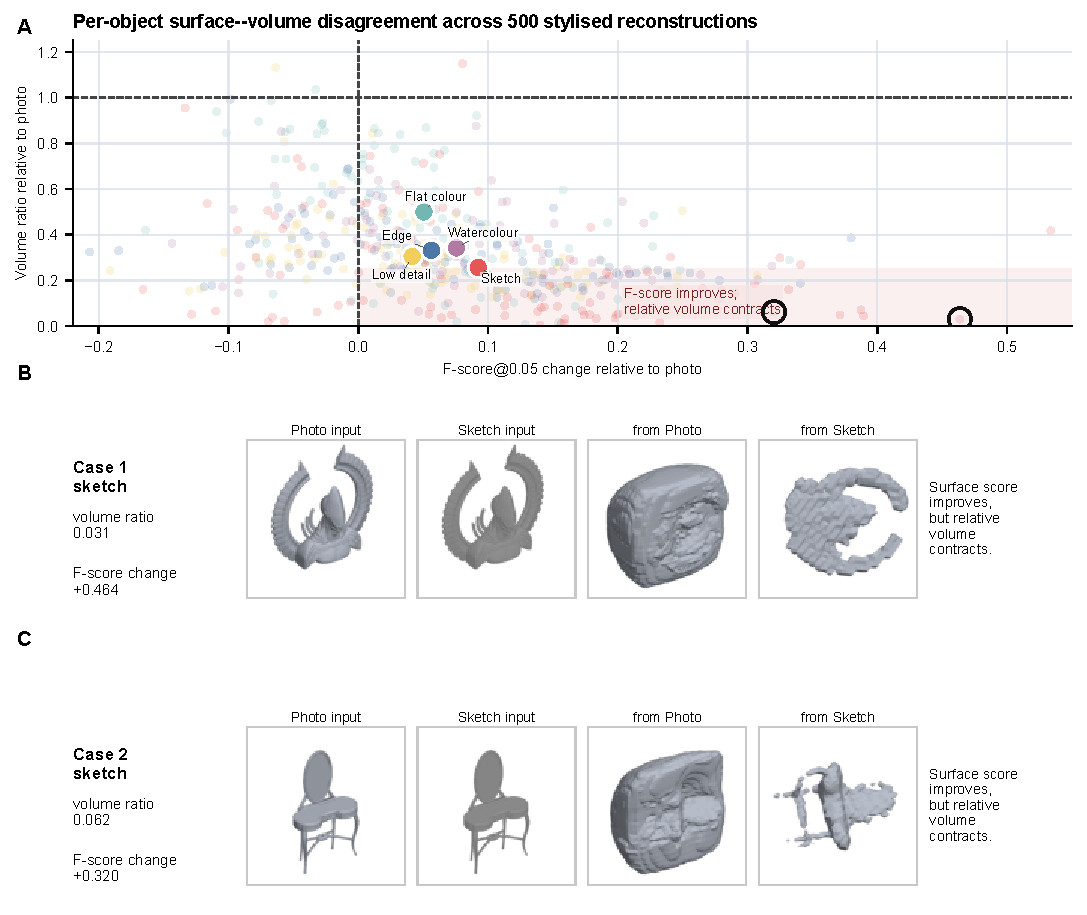
\includegraphics[width=\linewidth]{figures/fig3_metric_paradox_cases.pdf}
\caption{\label{fig:metricparadox}Per-object metric disagreement and representative cases. (A) Across 500 stylised reconstructions, many points fall in the region where F-score improves relative to the photo reconstruction while volume remains far below the photo baseline. Large filled points show unstratified style means, and outlined points mark the two visual cases. (B, C) In two sketch examples, F-score improves while the predicted mesh undergoes severe relative volumetric contraction.}
\end{figure}

The disagreement is most visible when F-score and volume are read together. All five style means improve F-score@0.05 in the unstratified analysis, so a surface-metric-only report could describe stylisation as beneficial. The volume ratios support the opposite interpretation for volumetric preservation. The same output can therefore be closer to the ground-truth surface sample under one metric while occupying much less volume than the paired photo output. Whether this constitutes lower usability requires task-specific or human evaluation, which the present benchmark does not provide.

One plausible explanation is that stylisation simplifies the evidence available to the model. A sketch or edge rendering may emphasise the visible contour and suppress texture that would otherwise create noisy or ambiguous local detail. This can help surface samples align with the visible object boundary. At the same time, the missing shading and interior evidence can weaken the model's inference about thickness and back-side geometry. The result is a mesh that is efficient at explaining the image from the observed view but incomplete as a volumetric object. The benchmark does not prove this mechanism directly, but the style-specific pattern is consistent with it.

\subsection{Surface-metric gains depend on photo-baseline quality}

Table~\ref{tab:baseline} separates the lower and higher halves of the photo-baseline F-score distribution. Volumetric contraction persists in both halves. In the higher-quality half, mean volume ratios range from 0.329 for low-detail to 0.707 for flat colour, and every value remains below one. The surface-metric pattern is much less stable. Mean F-score changes in the higher-quality half range from $-0.004$ to $+0.041$, compared with gains of $+0.089$ to $+0.164$ in the lower-quality half.

\begin{table}[!ht]
\caption{Post hoc sensitivity to photo-baseline quality. The lower and higher groups each contain 50 objects split at photo F-score@0.05 = 0.2368. The upper-quartile column contains the 25 strongest photo baselines.}
\label{tab:baseline}
\centering
\begin{tabular}{lrrrrr}
\toprule
Style & Low $r^V$ & High $r^V$ & Low $\Delta F$ & High $\Delta F$ & Top-quartile $\Delta F$ \\
\midrule
edge & 0.299 & 0.365 & 0.103 & 0.010 & -0.049 \\
flat & 0.293 & 0.707 & 0.089 & 0.012 & -0.018 \\
low-detail & 0.282 & 0.329 & 0.089 & -0.004 & -0.060 \\
sketch & 0.121 & 0.393 & 0.164 & 0.021 & -0.040 \\
watercolour & 0.258 & 0.427 & 0.110 & 0.041 & -0.014 \\
\bottomrule
\end{tabular}
\end{table}

The upper-quartile check makes the moderation clearer: mean F-score change is negative for every style among the 25 strongest photo reconstructions. The original aggregate result is therefore not evidence that stylisation generally improves surface reconstruction. Rather, stylisation can outperform a weak photo reconstruction under F-score while still producing a smaller output mesh. The volume result is the more stable finding; the surface-metric gain is baseline-conditioned.

\subsection{The effect persists at higher mesh-extraction resolution}

Table~\ref{tab:res128} reports the 30-object rerun with mesh extraction at resolution 128. The main pattern remains. All five stylised inputs reduce predicted volume, with mean ratios from 0.300 for low-detail to 0.588 for flat colour. Edge, low-detail, and watercolour again show strong z-extent reductions. Sketch still improves F-score@0.05 by 0.0685 while reducing mean volume to 0.340.

The higher-resolution run changes some magnitudes but not the conclusion. Flat colour improves to a volume ratio of 0.588 and nearly preserves z-extent, while edge and low-detail remain strongly compressed. Sketch still shows the key metric disagreement: F-score improves, Chamfer improves slightly, and volume remains far below the photo baseline. This is important because a resolution artefact would be expected to weaken substantially when the extraction grid becomes denser. Instead, the shrinkage remains statistically strong for all styles.

\begin{table}[!ht]
\caption{Robustness rerun with marching-cubes resolution 128 on 30 objects. The relative volumetric-contraction pattern remains under higher mesh-extraction resolution.}
\label{tab:res128}
\centering
\begin{tabular}{lrrrrr}
\toprule
Style & $\Delta$ Chamfer & $\Delta$ F@0.05 & Volume ratio & z-extent ratio & Volume $p$ \\
\midrule
edge & 0.0027 & 0.0301 & 0.377 & 0.461 & $2.98\times10^{-8}$ \\
flat & -0.0029 & 0.0293 & 0.588 & 0.962 & $6.56\times10^{-7}$ \\
low-detail & 0.0062 & 0.0191 & 0.300 & 0.412 & $3.73\times10^{-9}$ \\
sketch & -0.0024 & 0.0685 & 0.340 & 0.918 & $8.94\times10^{-8}$ \\
watercolour & -0.0020 & 0.0493 & 0.390 & 0.675 & $3.73\times10^{-9}$ \\
\bottomrule
\end{tabular}
\end{table}

\begin{figure}[!ht]
\centering
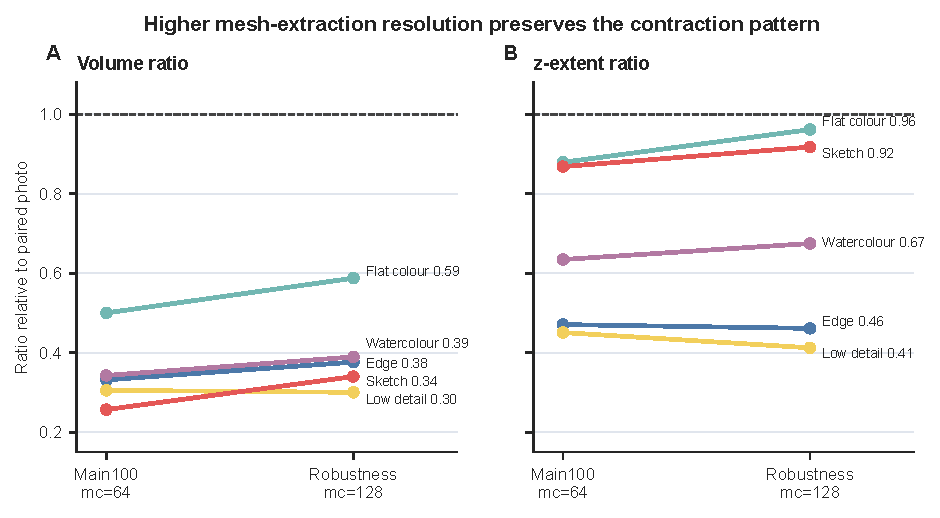
\includegraphics[width=\linewidth]{figures/fig4_res128_robustness.pdf}
\caption{\label{fig:res128}Robustness check under higher mesh-extraction resolution. The 30-object mc-resolution=128 rerun preserves the main relative volumetric-contraction pattern. Some styles recover part of the z-extent, but the predicted volume remains substantially below the paired photo baseline.}
\end{figure}

The rerun is smaller than the main experiment, so we treat it as robustness evidence rather than a replacement for the 100-object result. Still, it reduces a straightforward alternative explanation: the collapse is unlikely to be only an artefact of the lower mesh-extraction resolution used in the main run.

Taken together, the main experiment and the higher-resolution rerun support a stable claim about relative volumetric contraction in this TripoSR benchmark. The post hoc stratification adds an important qualification: apparent F-score improvements are strongest when the paired photo output is weak and disappear in the upper photo-quality quartile. The experiments therefore identify a robust geometric shift and a conditional metric disagreement rather than a universal benefit or failure of stylised input.

\section{Discussion}

The benchmark points to a practical risk in image-to-3D evaluation. Aggregate surface scores can make stylised inputs appear stronger even when TripoSR outputs occupy much less volume than their paired photo outputs. The new baseline analysis shows why this interpretation must be conditional: most apparent F-score gains arise where the photo reconstruction is weak. This distinction matters for computational design because a benchmark should not mistake recovery from a poor baseline for general robustness to stylisation.

The result also helps clarify what a benchmark for artistic image-to-3D should measure. Prior work has shown that specific artistic domains such as sketches, anime portraits, flat illustrations, and manuscript miniatures are challenging for current methods \parencite{sanghi2023sketchashape,chen2023panic3d,cong2025art3d,pallotto2026miniatures}. Our results suggest that the evaluation should not stop at whether the generated object looks plausible from the input view. A method can preserve the outline and still lose the volumetric fact of the object. Paired photo-versus-style comparisons make that loss visible.

For model developers, the findings suggest several remedies. First, benchmark reports should include volumetric and thickness-sensitive diagnostics alongside Chamfer and F-score. Second, style-stripping or geometry-preserving preprocessing should be evaluated not only by visual similarity but also by whether it restores volume and depth. Third, model selection for design workflows may need to depend on input style. A fast reconstruction model that is acceptable for photographs may need additional checks before it is used on sketches or flat illustrations.

The broader implication is that image-to-3D evaluation should be tied to the intended use of the output. If the goal is view synthesis, a source-view or near-view metric may be adequate. If the goal is an editable mesh, then the output must preserve more than appearance. It must preserve enough three-dimensional structure to support rotation, editing, texturing, and physical or procedural interpretation. Volume is a simple diagnostic for this requirement. It is not a complete solution, but it catches a failure that point metrics can miss. Z-extent provides a second coarse signal, especially for view-dependent flattening.

The benchmark also suggests a practical screening procedure. Before deploying an image-to-3D model in a design pipeline, users can test a small paired set of inputs that represent their actual reference material. The test does not require a large new dataset. A controlled set of known objects, rendered in the relevant style, can reveal whether the model is sensitive to abstraction. If the model loses volume under a style that is common in the workflow, the pipeline can add safeguards: ask for a photo-like reference, run a style-normalisation step, use a model trained for that input type, or flag the output for manual inspection.

For researchers developing new image-to-3D systems, the results argue for reporting paired style robustness rather than only aggregate benchmark scores. A model that performs well on photographs may still be brittle for sketches. A model that improves F-score under stylised inputs may still be unsuitable for asset generation if the improvement comes with volume loss. Reporting both point metrics and asset diagnostics would make such trade-offs visible. It would also help distinguish true geometric robustness from a metric improvement caused by simplified contours.

The study further shows why controlled synthetic rendering remains useful even when the target domain is artistic human input. Real drawings and illustrations are important, but they rarely come with exact 3D ground truth. Controlled stylisation of known 3D objects cannot replace real artwork, but it provides a bridge between ecological relevance and measurable geometry. It lets the evaluator ask a question that is difficult to answer with unpaired data: what changes when only the input style changes?

There is also a methodological lesson for future benchmarks. If a benchmark mixes many styles and object categories without pairing, the average score may hide where the model fails. A model could do well on flat illustrations of simple objects and poorly on edge renderings of thin objects, yet the aggregate number might appear acceptable. The paired structure used here supports a more diagnostic report. Each object can be treated as its own control, and each style can be analysed as a perturbation. This structure is especially useful when the expected failure is not random noise but a directional shift such as volume loss.

A second lesson concerns metric interpretation. Chamfer distance and F-score should not be discarded; they remain valuable for measuring sampled surface agreement. The problem is that they can be over-read. A lower Chamfer value does not necessarily mean that the generated mesh is a better design asset. It means that the sampled surface is closer under the chosen sampling and tolerance assumptions. For asset generation, this statement should be accompanied by diagnostics that describe whether the output still occupies a plausible three-dimensional region. Volume, z-extent, and related thickness measures are simple additions that make the interpretation less brittle.

The results also suggest why human inspection can be both necessary and unreliable as a sole evaluation method. A reviewer looking only at the source view may see a recognisable object and accept the reconstruction. The failure becomes more obvious when the mesh is rotated, when a cross-section is inspected, or when the object is used downstream. A benchmark should therefore make this hidden failure visible numerically before it reaches a user. Volumetric diagnostics are not a substitute for visual inspection, but they can decide which outputs deserve closer inspection.

\section{Limitations}

This study has several boundaries. We evaluate one primary image-to-3D baseline, TripoSR, so the results should not be stated as universal behaviour across all modern systems. The benchmark uses 100 curated Objaverse objects, which is sufficient for the observed paired statistical effect but not for broad category-level claims. A larger benchmark should stratify objects by shape family, concavity, symmetry, texture dependence, and component count. Such a study could identify which object properties make style-induced collapse more likely.

The style transformations are controlled proxies for artistic inputs; they do not cover the full diversity of human artwork. Real sketches can include construction lines, perspective errors, intentional exaggeration, ambiguous boundaries, or semantic conventions that are not reproduced by image filters. Real watercolour and concept art may also contain stylistic cues that are meaningful to humans but unfamiliar to a reconstruction model. The controlled proxy is useful for isolating style, but it should be complemented by studies on real artistic datasets.

The current study also reports mesh-level diagnostics and does not include a human usability study. Volume and z-extent are interpretable, but they are not direct measures of usefulness. A mesh can preserve volume while having poor topology, disconnected parts, or unusable surface detail. Conversely, a lower-volume reconstruction might still be acceptable for a decorative or low-poly asset. Future work should test whether volumetric diagnostics predict human judgements of editability, recognisability after rotation, and fabrication readiness.

The photo-baseline stratification is post hoc and should be treated as a sensitivity analysis rather than a pre-registered confirmatory test. Its median and upper-quartile thresholds are transparent and use only the paired photo F-score, but a larger benchmark should pre-specify baseline-quality strata and validate the moderation pattern on an independent object set.

Finally, the benchmark does not test mitigation strategies. We do not evaluate style-stripping, multi-view prompting, material-aware reconstruction, or newer textured models as fixes. This is a deliberate scope choice. The first step is to show that the metric gap exists under a controlled paired design. The next step is to test whether stronger models or preprocessing methods reduce the gap without sacrificing the benefits of artistic input.

\section{Conclusion}

We presented a paired benchmark for measuring how controlled stylised input transformations affect TripoSR reconstruction when the source 3D object is known. Across 100 curated Objaverse objects, all five style conditions reduce predicted mesh volume relative to paired photo outputs. A higher-resolution mesh-extraction rerun preserves this contraction pattern. Aggregate Chamfer and F-score gains occur, but they are concentrated among weak photo baselines and become negative for every style in the strongest photo-quality quartile.

The main lesson is that surface proximity and volumetric preservation are distinct, and their relationship depends on baseline quality. For image-to-3D systems used in computational design and 3D asset workflows, evaluation should therefore report paired volume and depth diagnostics together with conventional surface metrics and should stratify results by photo-baseline performance. Such reporting cannot replace task-specific human evaluation, but it prevents an aggregate surface score from hiding a systematic change in three-dimensional extent.

\section*{Data and code availability}

The aggregate result tables, analysis and figure-generation scripts, and selected-object manifest are included in the supplementary reproducibility package. Raw Objaverse assets are not redistributed because their reuse remains subject to the source licences. Object identifiers and recorded licences are provided so that eligible assets can be retrieved through Objaverse. The reproducibility package is available to editors and reviewers from the corresponding author and will be deposited in a persistent public repository with the accepted article.

\section*{Competing interests}

The authors declare no competing interests.

\printbibliography

\end{document}
